\documentclass{article}
\usepackage{amsmath}

\usepackage{float}
\usepackage{graphicx}


\begin{document}
\title{\textbf{FYS4150/FYS3150 - Project 2}}
\author{Ingvild Bergsbak, Oliver Hebnes and Erlend Ousdal}
\date{October 24}




\maketitle

\section{Abstract}

\section{Introduction}

\section{Theoretical Models and Technicalities}

For a circular orbit around the sun, the force between the sun the the earth is given by

$$F_G=\frac{M_{Earth}v^2}{r}=\frac{GM_{\odot}M_{Earth}}{r^2}$$

and we have that

$$v^2r=GM_{\odot}=\frac{4\pi^2\mathrm{AU}^3}{\mathrm{yr}^2}$$

which gives

$$F_G=\frac{4\pi^2\mathrm{AU}^3M_{Earth}}{r^2\mathrm{yr}^2}$$

Newton's second law gives

$$\mathbf{r}''=\mathbf{a}=\frac{F_G}{M_{Earth}}=\frac{4\pi^2\mathrm{AU}^3M_{Earth}}{r^2\mathrm{yr}^2M_{Earth}}=\frac{4\pi^2\mathrm{AU}^3}{r^2\mathrm{yr}^2}$$


\section{Results and Discussion}

\subsection{Earth-sun system}
It was found that the initial velocity that gives a circular orbit is $2\pi$, as given in \ref{jordensbane}.
\begin{figure}[H]
  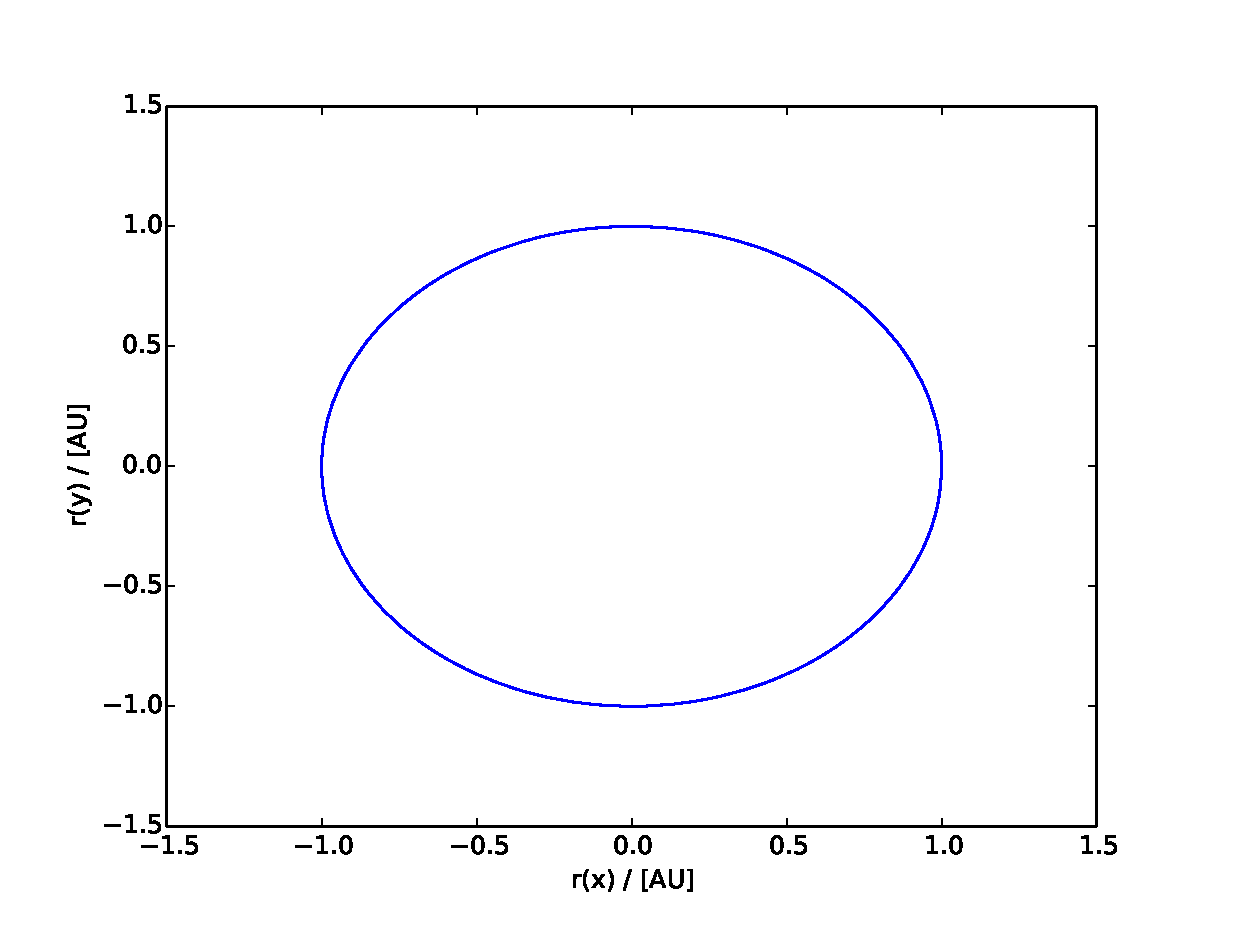
\includegraphics[scale=0.6]{3c_jordensbane_verlet_n10e6.eps}
  \caption{The Earth in a circular orbit around the origin (the sun) with intial velocity $2\pi$ in positive vertical direction. This is done by using Veilet's algorithm with $10^6$ integration points.}
  \label{jordensbane}
\end{figure}

\begin{table}[H]
    \centering
    \begin{tabular}{|l|c|c|c|r|}
    \hline
     $n$ & Verlet error  & Euler error & Time Verlet & Time Euler\\
     \hline
      $10^3$  & $1.96\cdot10^{-10}$  & $7.77\cdot10^{-2}$ & $ 4.90 (30) \cdot 10^{-3}$ & $ 4.44 (28) \cdot 10^{-3}$\\
      $10^4$  & $4.09\cdot10^{-14}$  & $7.90\cdot10^{-3}$ & $ 1.42 (27) \cdot 10^{-2}$ & $ 9.90 (40) \cdot 10^{-3}$\\
      $10^5$  & $5.22\cdot10^{-14}$  & $7.90\cdot10^{-4}$ & $ 9.81 (29) \cdot 10^{-2}$ & $ 6.42 (36) \cdot 10^{-2}$\\
      $10^6$  & $2.05\cdot10^{-13}$  & $7.89\cdot10^{-5}$ & $ 8.96 (35) \cdot 10^{-1}$ & $ 5.28 (45) \cdot 10^{-1}$\\
      \hline
    \end{tabular}
    \caption{Testing the stability and time used for Euler's algorithm and Verlet's algorithm.}
    \label{stability}
\end{table}

When comparing Euler's forward algorithm with Veilet's algorithm, it is clear that Verlet is a very accurate method compared to Euler's forward algorithm. Even if Verlet uses a bit more time than Verlet, we see that it is a small sacrifise for a much greater accuracy for our solar system.   
\section{Conclusion}


\end{document}
